The product will have 3 layers: The mobile application layer, web application layer, and database layer. This section will describe what each of these layers do.

\begin{figure}[h!]
	\centering
 	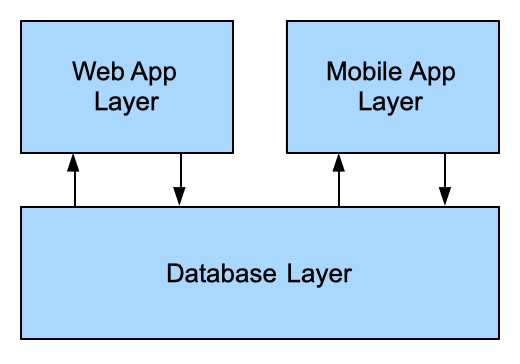
\includegraphics[width=0.60\textwidth]{images/architectural_layer_diagram.png}
 \caption{The architectural layer diagram of Swift Scan}
\end{figure}

\subsection{Mobile Application Layer Description}
The mobile app will contain 3 tabs: profile, scan, and saved. The profile tab will ensure that all user settings are saved and can be synced with the web app. The scan tab will allow users to scan products using the camera and view information about them. If they choose to save the product information, it will be stored in the saved tab. The saved tab lists every product save by the user. These products can be sorted by type of alcohol or any other category. The user can also make collections with products of their choice. 

\subsection{Web Application Description}
The web app will include a profile tab and saved tab with the same features as the mobile app. The information will be synced from the mobile app via the database system so that the user can access their products anywhere. When the web page is refreshed, a request will be sent to the database for the up-to-date information on the user.

\subsection{Database Layer Description}
The database system is the driving force of the project. When a user scans a product, the database will be queried for the barcode number. Information such as name, brand, price, ABV, type, country, and category will be returned the user. In addition, the database will store the information of all users and will be monitored by the maintenance team. To login, the user will enter their username and password which will be queried in the database to confirm their identity and all of their setting setting will be returned. 
